\documentclass[12pt,draftcls,onecolumn]{IEEEtran}
%\documentclass[onecolumn]{IEEEtran}

\usepackage{amsmath}
\usepackage{amsthm}
\usepackage{amssymb}  % assumes amsmath package installed
\usepackage{algorithmic}
\usepackage{algorithm}
\usepackage{cite}
\usepackage{color}
\usepackage{comment}
\usepackage{epsfig}
\usepackage{float}
\usepackage{graphicx}
\usepackage{multicol}
\usepackage{subfigure}
\usepackage{setspace}
\usepackage{comment}
\usepackage{subfig} % for subfigures
\usepackage{caption}



\newtheorem{theorem}{Theorem}[section]
\newtheorem{lemma}[theorem]{Lemma}
\newtheorem{proposition}[theorem]{Proposition}
\newtheorem{corollary}[theorem]{Corollary}
\newtheorem{remark}[theorem]{remark}

\begin{document}

\title{Report on the Path Planning of Webot Satisficing Experiment }


\author{  Min Zheng \\  \today}

\date{\today}

% make the title area
\maketitle



%\IEEEpeerreviewmaketitle

%%%%%%%%%%%%%%%%%%%%%%%%%%%%%%%%%%%%%%%%%%%%%%%%%%%%%%%%%%%%%%%%%%%%%%%%%%%%%%
This project considers the integrated navigation and control of an unmanned ground vehicle(UGV) deployed to visually classify multiple targets in an obstacle-populated environment. 
This report describes the setup of the path planning problem and proposes some potential problems and plans. 

\section{Workspace construction} 

The workspace is the same as the one used for active satisficing human studies. 
The UGV and 30 target objects are in the same environment that consists of four rooms, denoted as the region-of-interest (ROI).
Similar to the human studies, there are 30 targets, denoted as $\mathcal{T} = \{\mathcal{T}_i; i = 1,2,...30; \mathcal{T} \subset W \}$.
The targets are considered as points.
A two-dimensional representation from the webot environment was extracted, and the workspace is constructed in MatLab, as shown in the figure below  (Figure \ref{fig:2}). 
The construction of workspace is built in an object oriented manner with classes of obstacles, targets and robot, each has properties and functionalities.  




\begin{figure}[p]
\centering
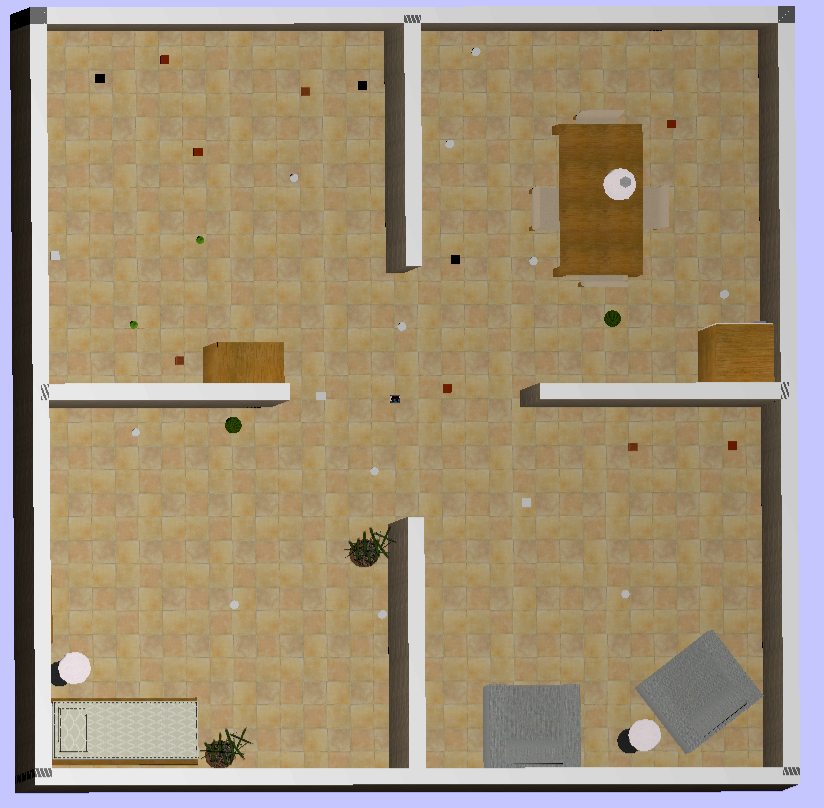
\includegraphics[width=10cm]{figures/webotTop}
  \caption{Top view of the webot environment}
  \label{fig:1}
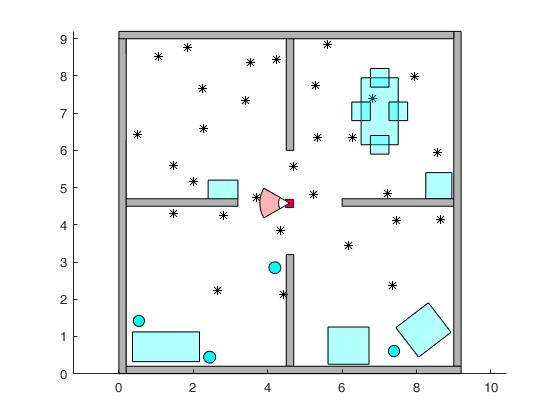
\includegraphics[width=16cm]{figures/matlabExtraction}
  \caption{2D representation built in MatLab. Obstacles are represented by colored regions, and targets represented by the stars. The UGV is  the red square, while its FOV is the red area within the fan shape.}
  \label{fig:2}
\end{figure}



\clearpage


\section{FOV and C-Target generation} 


The UGV sensor in the webot environment has platform geometry $\mathcal{A}$, and FOV geometry $S \subset \mathbb{R}^2 $. 
The dimension of UGV is 0.12m x 0.10m in 2D.
Its translation step is 0.01m, and rotation step is $\pi/12$ .
The UGV configuration is described in  (Figure \ref{fig:1}).
The configuration vector is defined as $q \equiv [x  \quad  y  \quad  \theta]^T$



In order to combine with Zeyu's visual classification project, the FOV was determined based on requirement of  images taken. 
A successful classification requires the image to be taken within a minimum and a maximum distance, denoted by $d_{min}$ and  $d_{max}$. 
In human tests, the open angle of FOV for the on board camera is $\alpha =\pi/3 $. 
Therefore the same  $\alpha$ is used here.
Also, in the visual classification problem, Ryan took all the pictures from 0.3m.
If the picture is taken less than that distance, the target object is not guaranteed to be completely within the camera view.
Meanwhile, in the human tests software setup, the robot must be within 1m from the target to  measure or classify.
In such manner, the range of distance from target is conservatively set within $d_{min} = 0.3m$ and  $d_{max}=0.8 m$.
In order to better work with the visual classification, these parameters, especially $d_{max}$ may be subject to changes due to the highly sensitive manner of visual classifier. 
For example, it may be affected by whether the visual classifier allows multiple objects to appear in the view. 

\begin{figure}
 \centering
  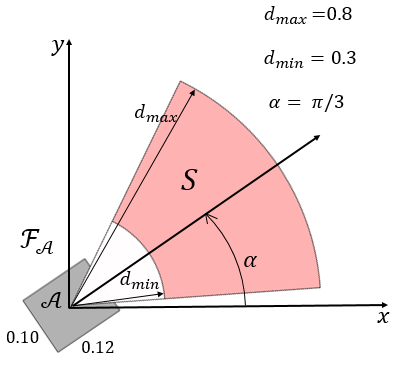
\includegraphics[width=10cm]{figures/FOV}
  \caption{Configuration and FOV of the UGV.}
  \label{fig:1}
\end{figure}







\begin{figure*}[htp]
  \centering
  \subfigure[ $\mathcal{C}_{free}$  given robot configuration]{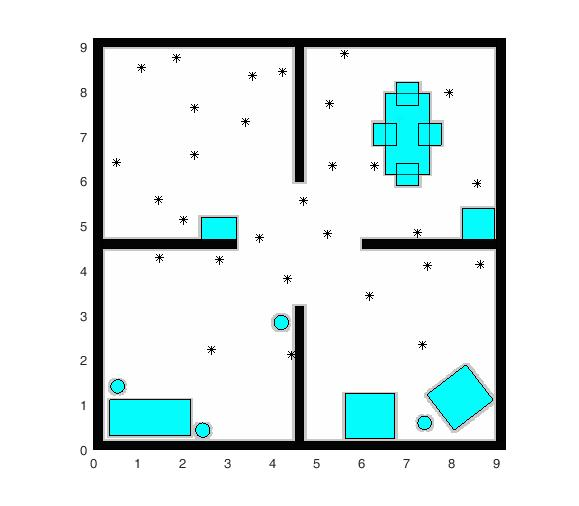
\includegraphics[width=12cm]{figures/Cfree}}\quad
  \subfigure[Zoomed-in of above figure]{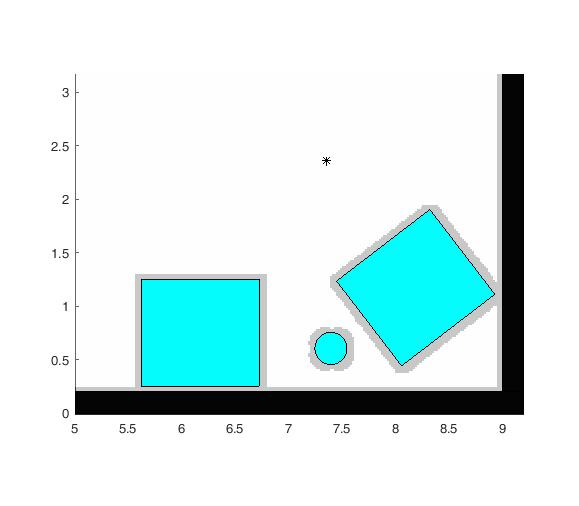
\includegraphics[width=12cm]{figures/Cfree_zoom}}
  \caption{ $\mathcal{C}_{free}$  of the given world map denoted by white region. Grey area is not in  $\mathcal{C}_{free}$ }
  \label{fig:8}
\end{figure*}




Currently, the  $\mathcal{C}_{free}$ is defined with a non-rotating UGV body (Figure \ref{fig:8}).
So that the UGV can only stand on the points in $\mathcal{C}_{free}$, with a  $\theta =0 $ or $\theta = pi$.


Assume that the UGV camera can freely rotate.
C-Target is defined so that the target $\mathcal{T}_i$ in $\mathcal{W}$ maps  in the robot's configuration space  $\mathcal{C}_{free}$ to the C-target region  $\mathcal{CT}_i = \{q \in \mathcal{C}_{free}    |    \mathcal{S}(q) \cap \mathcal{T}_i  \neq  \emptyset \}$.
The computation of C-target is illustrated for a single target in Figure \ref{fig:4}.
In (a), the robot is within C-target, since the target is in the robot's FOV when it faces $-pi/2$.
In (b), the robot is not in C-target, and it can not detect the target no matter how it rotates at its current position. 



\begin{figure*}[htp]
  \centering
  \subfigure[robot is in C-target]{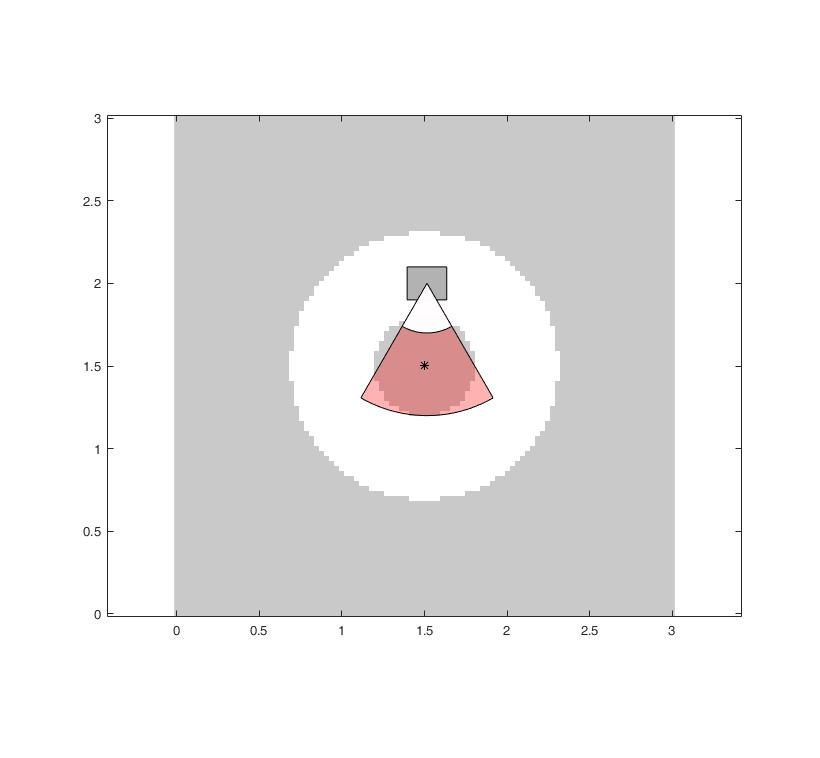
\includegraphics[width=12cm]{figures/oneTargetTrue}}\quad
  \subfigure[robot is not in C-target]{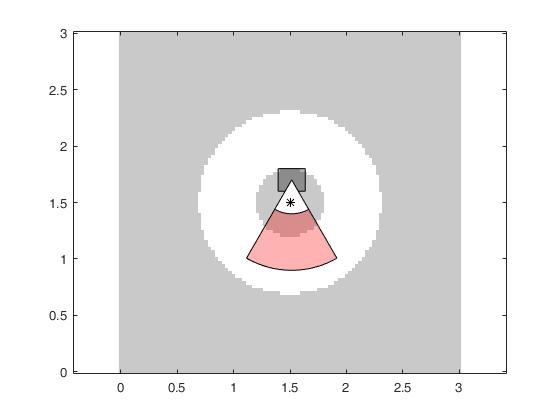
\includegraphics[width=12cm]{figures/oneTargetFalse}}
  \caption{Example of C-target with one target. C-target denoted by white area, and the star denotes the target. The target must fall in the red region(robot FOV) to be classified or measured. In both examples, the UGV is facing $\theta = -pi/2$}
  \label{fig:4}
\end{figure*}


Then, at every location in $\mathcal{C}_{free}$ , as the robot camera rotates freely but no any target is in its FOV, then such location is excluded from C-target.
The visibility problem is introduced to deal with the case that the camera view is blocked by obstacles.
That is, a target must be in the FOV of the given UGV configuration, and at the same time, if a line is drawn between the robot and the target, such a line must not cross any obstacle, demonstrated in  (Figure \ref{fig:7}).
If this criteria is met, such a UGV configuration is defined as in the  $\mathcal{C}_{target}$.
The C-Target is plotted in the workspace (Figure \ref{fig:5}).
C-Target is denoted by white, where the rest region in $\mathcal{C}_{free}$ is grey. 








\begin{figure}
 \centering
  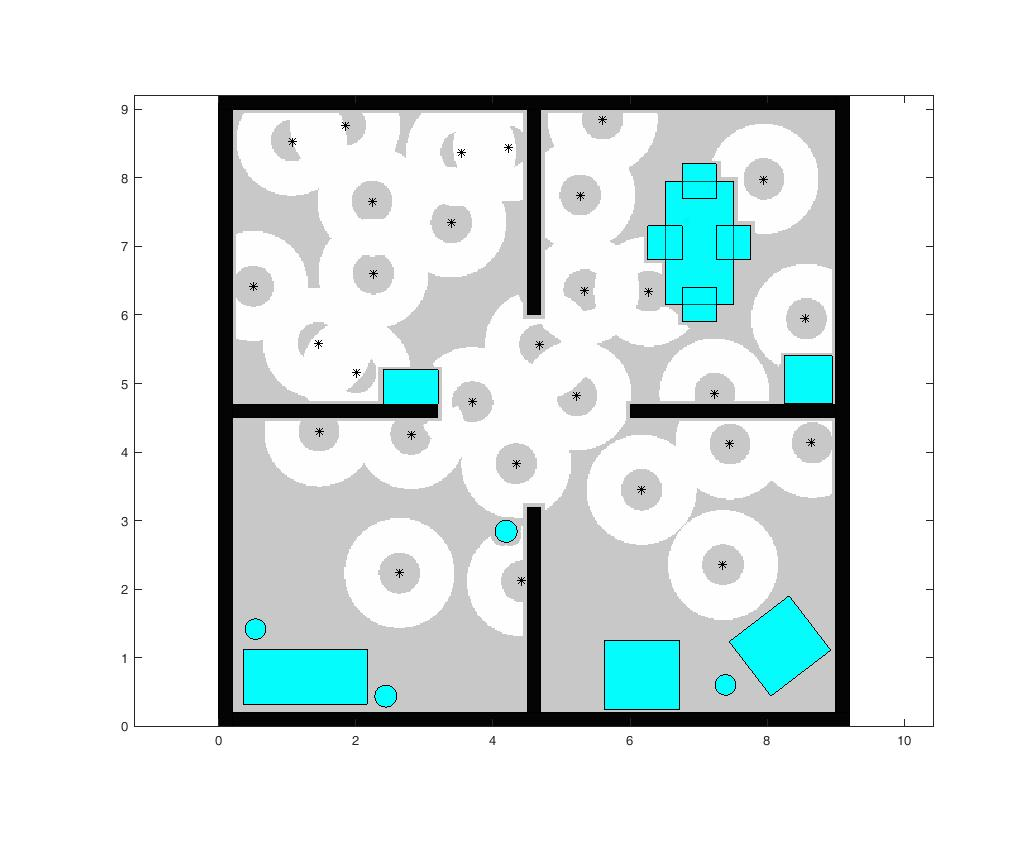
\includegraphics[width=18cm]{figures/CTarget}
  \caption{C-Target is denoted by white, where the rest region in $\mathcal{C}_{free}$ is grey.}
  \label{fig:5}
\end{figure}


\begin{figure}
 \centering
  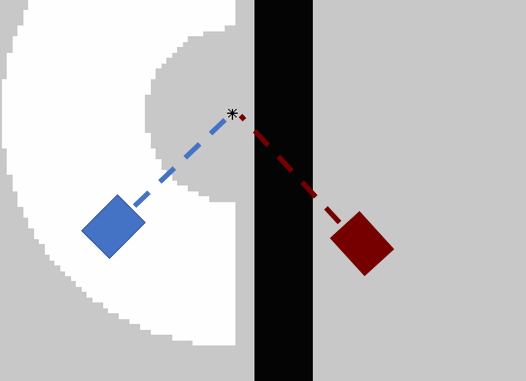
\includegraphics[width=5cm]{figures/visibility_eg}
  \caption{Example of visibility problem handling for a target near the wall. The blue and red rectangles denote the UGV configuration. The dash line denotes the direction the robot is facing. It is also used in the visibility handling. The blue configuration is in C-Target, but the red is not since its view is blocked by the obstacle.}
  \label{fig:7}
\end{figure}







\end{document}
